\documentclass{article}

\usepackage{pandekten}

\usepackage{dashrule}

\makeatletter
\newcommand*{\shifttext}[1]{%
  \settowidth{\@tempdima}{#1}%
  \hspace{-\@tempdima}#1%
}
\newcommand{\plabel}[1]{%
\shifttext{\textbf{#1}\quad}%
}
\newcommand{\prule}{%
\begin{center}%
\hdashrule[0.5ex]{.99\linewidth}{1pt}{1pt 2.5pt}%
\end{center}%
}

\makeatother

\setlength{\parindent}{0pt}

\title{Assignment 1}
\author{Ze Chen}

\begin{document}

\maketitle

\plabel{1 (a)}%
The 5 lowest lying states are given below.
\begin{center}
    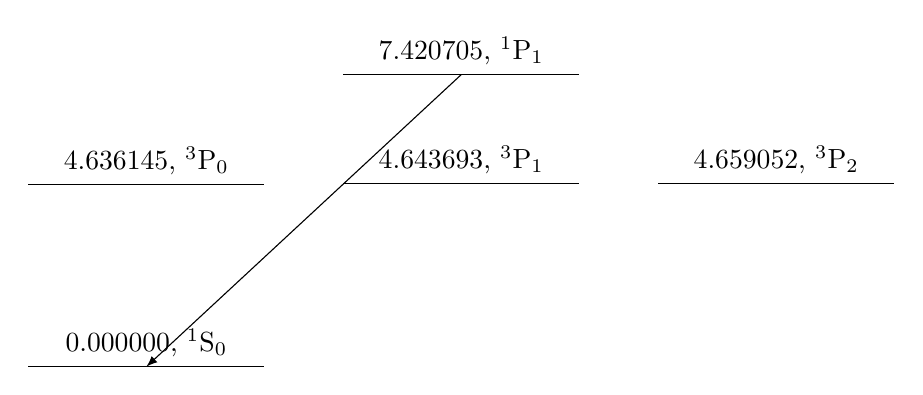
\begin{tikzpicture}[yscale=0.5]
        \draw[] (0, 0) -- (3, 0) node[midway,above]{\SI{0.000000}{\eV}, $\mathrm{^1S_0}$};
        \draw[] (0, 4.636145) -- (3, 4.636145) node[midway,above] {\SI{4.636145}{\eV}, $\mathrm{^3P_0}$};
        \draw[] (4, 4.643693) -- (7, 4.643693) node[midway, above]{\SI{4.643693}{\eV}, $\mathrm{^3P_1}$};
        \draw[] (8, 4.659052) -- (11, 4.659052) node[midway,above]{\SI{4.659052}{\eV}, $\mathrm{^3P_2}$};
        \draw[] (4, 7.420705) -- (7, 7.420705) node[midway,above]{\SI{7.420705}{\eV}, $\mathrm{^1P_1}$};
        %
        \draw[-latex] (5.5, 7.420705) -- (1.5, 0);
        %\draw[-latex] (5.5, 4.643693) to[out=-110,in=-70] (1.5, 4.636145);
        %\draw[-latex] (9.5, 4.659052) to[out=-110,in=-70] (5.5, 4.643693);
    \end{tikzpicture}
\end{center}

\plabel{(b)}%
The selection rule is given by
\begin{align*}
    \Delta J &= \qty{0,\pm 1}, \\
    \Delta M_J &= \qty{0, \pm 1}, \\
    \Delta S &= 0, \\
    \Delta L &= \qty{0,\pm 1}, \\
    \text{but no } L &= 0 \rightarrow L = 0 \text{ transitions}, \\
    \text{Laporte rule } (-1)^{\Delta \sum_i l_i} &\neq 1.
\end{align*}

\plabel{(c)}%
The only stable isotope is \ce{^{27}Al}, where $I=5/2$.
The F-levels are given below.
\begin{center}
    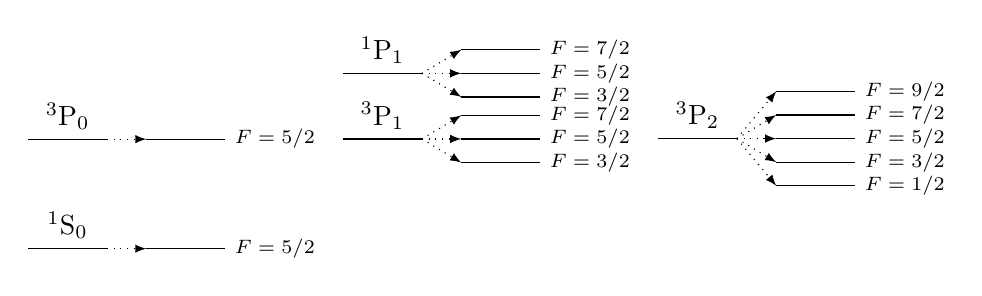
\begin{tikzpicture}[yscale=0.3]
        \draw[] (0, 0) -- (1, 0) node[midway,above]{$\mathrm{^1S_0}$};
        \draw[dotted,-latex] (1,0) --++(0.5,0);
        \draw (1,0) ++(0.5,0) --++(1,0) node[right] {\scriptsize $F=5/2$};
        %
        \draw[] (0, 4.636145) -- (1, 4.636145) node[midway,above] {$\mathrm{^3P_0}$};
        \draw[dotted,-latex] (1,4.636145) --++(0.5,0);
        \draw (1,4.636145) ++(0.5,0) --++(1,0) node[right] {\scriptsize $F=5/2$};
        %
        \draw[] (4, 4.643693) -- (5, 4.643693) node[midway, above]{$\mathrm{^3P_1}$};
        \draw[dotted,-latex] (5,4.643693) --++(0.5,0);
        \draw[dotted,-latex] (5,4.643693) --++(0.5,1);
        \draw[dotted,-latex] (5,4.643693) --++(0.5,-1);
        \draw (5,4.643693) ++(0.5,0) --++(1,0) node[right] {\scriptsize $F=5/2$};
        \draw (5,4.643693) ++(0.5,1) --++(1,0) node[right] {\scriptsize $F=7/2$};
        \draw (5,4.643693) ++(0.5,-1) --++(1,0) node[right] {\scriptsize $F=3/2$};
        %
        \draw[] (8, 4.659052) -- (9, 4.659052) node[midway,above]{$\mathrm{^3P_2}$};
        \draw[dotted,-latex] (9,4.659052) --++(0.5,0);
        \draw[dotted,-latex] (9,4.659052) --++(0.5,1);
        \draw[dotted,-latex] (9,4.659052) --++(0.5,-1);
        \draw[dotted,-latex] (9,4.659052) --++(0.5,2);
        \draw[dotted,-latex] (9,4.659052) --++(0.5,-2);
        \draw (9,4.659052) ++(0.5,0) --++(1,0) node[right] {\scriptsize $F=5/2$};
        \draw (9,4.659052) ++(0.5,1) --++(1,0) node[right] {\scriptsize $F=7/2$};
        \draw (9,4.659052) ++(0.5,-1) --++(1,0) node[right] {\scriptsize $F=3/2$};
        \draw (9,4.659052) ++(0.5,2) --++(1,0) node[right] {\scriptsize $F=9/2$};
        \draw (9,4.659052) ++(0.5,-2) --++(1,0) node[right] {\scriptsize $F=1/2$};
        %
        \draw[] (4, 7.420705) -- (5, 7.420705) node[midway,above]{$\mathrm{^1P_1}$};
        \draw[dotted,-latex] (5,7.420705) --++(0.5,0);
        \draw[dotted,-latex] (5,7.420705) --++(0.5,1);
        \draw[dotted,-latex] (5,7.420705) --++(0.5,-1);
        \draw (5,7.420705) ++(0.5,0) --++(1,0) node[right] {\scriptsize $F=5/2$};
        \draw (5,7.420705) ++(0.5,1) --++(1,0) node[right] {\scriptsize $F=7/2$};
        \draw (5,7.420705) ++(0.5,-1) --++(1,0) node[right] {\scriptsize $F=3/2$};
    \end{tikzpicture}
\end{center}

\prule

\plabel{2 (a)}%
With $\vb{B} = B \hat{\vb{z}}$, the Hamiltonian in matrix form with basis
\[ \qty(\ket{m_J=+\frac{1}{2}},\ket{m_J=-\frac{1}{2}}) \otimes \qty(\ket{m_I=+\frac{1}{2}},\ket{m_I=-\frac{1}{2}}) \]
is given by
\begin{gather*}
    H = g \mu_{\mathrm{B}} B \frac{1}{2} \sigma_z \otimes \sigma_0 + g_{\mathrm{n}} \mu_{\mathrm{N}} B \frac{1}{2} \sigma_0 \otimes \sigma_z + A \frac{1}{4} \sum_{i=x,y,z} \sigma_i\otimes \sigma_i \\
    = \arraycolsep=-17pt \begin{pmatrix}
        \frac{1}{4} A + \frac{1}{2} g\mu_{\mathrm{B}} B + \frac{1}{2} g_{\mathrm{n}} \mu_{\mathrm{N}} B & & & \\
        & -\frac{1}{4} A + \frac{1}{2} g\mu_{\mathrm{B}} B - \frac{1}{2} g_{\mathrm{n}} \mu_{\mathrm{N}} B & \frac{1}{2} A \\
        & \frac{1}{2} A & -\frac{1}{4} A - \frac{1}{2} g\mu_{\mathrm{B}} B + \frac{1}{2} g_{\mathrm{n}} \mu_{\mathrm{N}} B \\
        & & & \frac{1}{4} A - \frac{1}{2} g\mu_{\mathrm{B}} B - \frac{1}{2} g_{\mathrm{n}} \mu_{\mathrm{N}} B
    \end{pmatrix}.
\end{gather*}

\plabel{(b)}%
The first two coefficients are given by
\[ g\mu_{\mathrm{B}} = 2.002 \times \mu_{\mathrm{B}} = h\times \SI{28.02}{\giga\hertz\per\tesla}, \]
and
\[ g_{\mathrm{n}} \mu_{\mathrm{N}} = 0.4923 \times \mu_{\mathrm{N}} = h \times \SI{3.753e-3}{\giga\hertz\per\tesla}. \]

\plabel{(c)}%
The plot is given below.
\begin{center}
    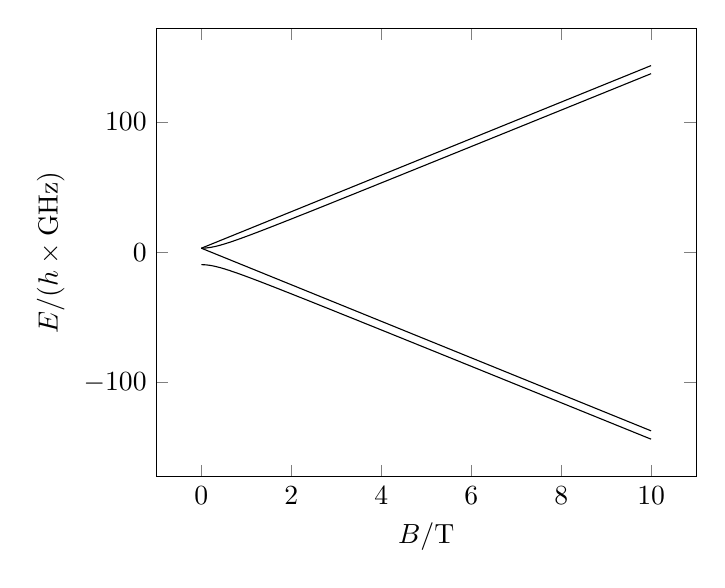
\begin{tikzpicture}
        \begin{axis}[domain=0:10,samples=100,xlabel=$B/\mathrm{T}$,ylabel=$E/(h\times \mathrm{GHz})$]
            \addplot[] {3.15 - 14.0119*x};
            \addplot[] {0.5*(-6.3 - sqrt(158.76 + 784.91 * x^2))};
            \addplot[] {3.15 + 14.0119*x};
            \addplot[] {0.5*(-6.3 + sqrt(158.76 + 784.91 * x^2))};
        \end{axis}
    \end{tikzpicture}
\end{center}

\plabel{(d)}%
The space generated by
\[ \qty{\ket{F=0,F_z=0}, \ket{F=1,F_z=0}} \]
has relative energy shift $\delta \Delta E = \bigO(B^2)$, where
\begin{align*}
    \Delta E &= \sqrt{A^2 + B^2(g \mu_{\mathrm{B}} - g_{\mathrm{n}} \mu_{\mathrm{N}})^2} \\
    &\approx A + \frac{(g \mu_{\mathrm{B}} - g_{\mathrm{n}} \mu_{\mathrm{N}})^2}{2A} B^2
\end{align*}
where
\[ \frac{(g \mu_{\mathrm{B}} - g_{\mathrm{n}} \mu_{\mathrm{N}})^2}{2A} = h\times \SI{31.15}{\giga\hertz\per\square\tesla}. \]

\prule

\plabel{3 (1)}%
The primary system is \ce{Al+} and the ancilla system is \ce{Be+}.
This method mitigates the effects of noise and perturbations, and provides real-time measurement feedback, which can further enhance detection efficiency.
Moreover, short life of $^2\mathrm{P}_{3/2}$ state of \ce{Be+} allows multiple measurements and could therefore reduce error.

\plabel{(2)}%
$^1\mathrm{P}_1 \rightarrow ^1\mathrm{S}_0$: \SI{167.078}{\nano\meter},
$^3\mathrm{P}_0 \rightarrow ^1\mathrm{S}_0$: \SI{267.429}{\nano\meter}.

\plabel{(3)}%
Step 0: Initial state $(\alpha\ket{\downarrow}_{\ce{Al}} + \beta\ket{\uparrow}_{\ce{Al}})\ket{\downarrow}_{\ce{Be}}\ket{0}_{\mathrm{m}}$.
\par
Step 1: After a $\pi$ pulse, to
\[ \alpha\ket{^3\mathrm{P}_1}_{\ce{Al}}\ket{\downarrow}_{\ce{Be}}\ket{1}_{\mathrm{m}} + \beta\ket{\uparrow}_{\ce{Al}}\ket{\downarrow}_{\ce{Be}}\ket{0}_{\mathrm{m}}. \]
\ce{Al+} and motion are entangled.
\par
Step 2: After a $\pi$ pulse, to
\[ \alpha\ket{^3\mathrm{P}_1}_{\ce{Al}}\ket{\uparrow}_{\ce{Be}}\ket{0}_{\mathrm{m}} + \beta\ket{\uparrow}_{\ce{Al}}\ket{\downarrow}_{\ce{Be}}\ket{0}_{\mathrm{m}}. \]
\ce{Al+} and \ce{Be+} are entangled.

\plabel{(4)}%
Step 0: Initial state $(\alpha\ket{\downarrow}_{\ce{Al}} + \beta\ket{\uparrow}_{\ce{Al}})\ket{\downarrow}_{\ce{Be}}\ket{1}_{\mathrm{m}}$.
\par
Step 1: After a $\pi$ pulse, to
\[ \alpha\ket{^3\mathrm{P}_1}_{\ce{Al}}\ket{\downarrow}_{\ce{Be}}\ket{2}_{\mathrm{m}} + \beta\ket{\uparrow}_{\ce{Al}}\ket{\downarrow}_{\ce{Be}}\ket{1}_{\mathrm{m}}. \]
\par
Step 2: After a $\pi$ pulse, to
\[ \alpha\ket{^3\mathrm{P}_1}_{\ce{Al}}\ket{\uparrow}_{\ce{Be}}\ket{1}_{\mathrm{m}} + \beta\ket{\uparrow}_{\ce{Al}}\ket{\uparrow}_{\ce{Be}}\ket{0}_{\mathrm{m}}. \]
Therefore, measurement on $\beta$ always yields $\ket{\uparrow}$.

\plabel{(5)}%
Solving $e^{-\mu_1}\mu_1^{n^*} = e^{-\mu_2}\mu_2^{n^*}$ for $n^*$ we find $n^*\approx \num{3.64}$.
\begin{center}
    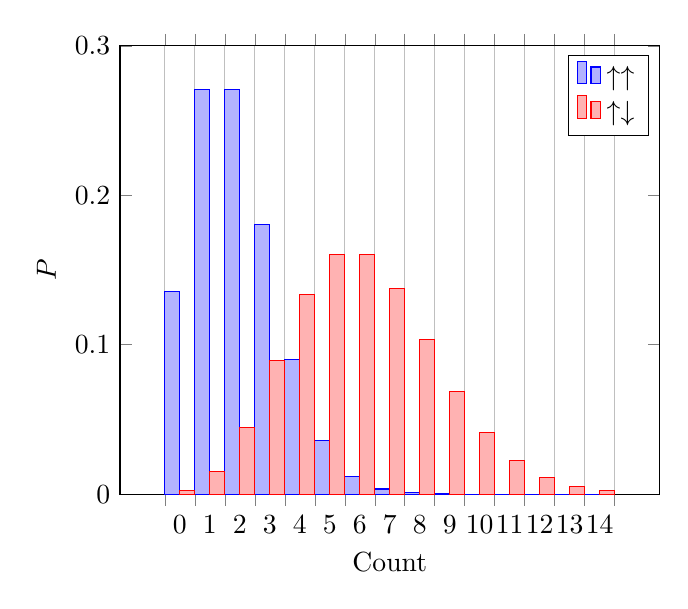
\begin{tikzpicture}
        \begin{axis}[ybar interval, ymax=0.3,ymin=0,xlabel=Count,ylabel=$P$]
        \addplot coordinates {
            (0,0.135335)
            (1,0.270671)
            (2,0.270671)
            (3,0.180447)
            (4,0.0902235)
            (5,0.0360894)
            (6,0.0120298)
            (7,0.00343709)
            (8,0.000859272)
            (9,0.000190949)
            (10,0.0000381899)
            (11,0.00000694361)
            (12,0.00000115727)
            (13,0.000000178041)
            (14,0.0000000254345)
            (15,0.00000000339126)
        };
        \addplot coordinates {
            (0,0.00247875)
            (1,0.0148725)
            (2,0.0446175)
            (3,0.0892351)
            (4,0.133853)
            (5,0.160623)
            (6,0.160623)
            (7,0.137677)
            (8,0.103258)
            (9,0.0688385)
            (10,0.0413031)
            (11,0.022529)
            (12,0.0112645)
            (13,0.00519899)
            (14,0.00222814)
            (15,0.000891256)
        };
        \legend{$\ket{\uparrow\uparrow}$,$\ket{\uparrow\downarrow}$}
        \end{axis}
    \end{tikzpicture}
\end{center}
The Bayesian approach is given by
\begin{align*}
    \operatorname{P}(\ket{\uparrow\uparrow}|m) &= \frac{\operatorname{P}(m|\ket{\uparrow\uparrow})}{\operatorname{P}(m|\ket{\uparrow\uparrow})+\operatorname{P}(m|\ket{\uparrow\downarrow})} \\
    &= \frac{e^{-\mu_1}\mu_1^m}{e^{-\mu_1}\mu_1^m + e^{-\mu_2}\mu_2^m}.
\end{align*}

\begin{center}
    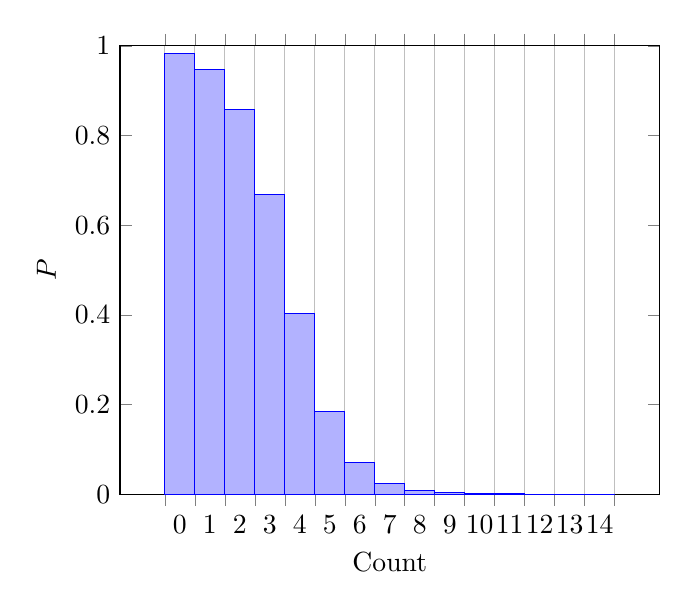
\begin{tikzpicture}
        \begin{axis}[ybar interval, ymax=1,ymin=0,xlabel=Count,ylabel=$P$]
        \addplot coordinates {
            (0,0.982014)
            (1,0.947915)
            (2,0.858486)
            (3,0.66911)
            (4,0.402647)
            (5,0.183463)
            (6,0.0696762)
            (7,0.0243568)
            (8,0.00825294)
            (9,0.0027662)
            (10,0.00092377)
            (11,0.000308113)
            (12,0.000102725)
            (13,0.0000342442)
            (14,0.000011415)
            (15,0.00000380502)
        };
        \end{axis}
    \end{tikzpicture}
\end{center}

At $m\approx n^*$, the probabilities for $\ket{\uparrow\uparrow}$ and $\ket{\uparrow\downarrow}$ to yield $m$ photons are close to each other, and therefore $P\approx \num{0.5}$.

\plabel{(6)}%
$t = -\tau' \ln (1-P) = -\SI{21}{\second}\times \ln(1-\SI{99.99}{\percent}) = \SI{193.4}{\second}$.

\prule

\plabel{5 (1)}%
The beams $\sigma^\pm_\parallel$ (frequency $f_{\mathrm{L}} - f_0$) and $\sigma^\mp$ (frequency $f_{\mathrm{L}}$) are used to drive the single qubit gate since their frequency matches (up to $\Delta$) $\ket{\uparrow} \rightarrow 4P_{1/2}$ and $\ket{\downarrow} \rightarrow 4P_{1/2}$, respectively.
\par
The beams $\sigma^\pm$ (frequency $f_{\mathrm{L}} - f_{z} - \delta_{\mathrm{g}}$) and $\sigma^\mp$ (frequency $f_{\mathrm{L}}$) because their energy difference $f_{z} + \delta_{\mathrm{g}}$ excites the vibration mode of frequency $f_z$ for $\ket{\Uparrow\Downarrow}$ and $\ket{\Downarrow\Uparrow}$.

\plabel{(2)}%
The fidelity could be written as
\[ F = \frac{1}{2}(P_{\Uparrow\Uparrow} + P_{\Downarrow\Downarrow}) + \abs{\rho_{\Uparrow\Uparrow,\Downarrow\Downarrow}}. \]
The parity
\[ P(\varphi) = P_{\Downarrow\Downarrow}(\varphi) + P_{\Uparrow\Uparrow}(\varphi) - P_{\Uparrow\Downarrow}(\varphi) - P_{\Downarrow\Uparrow}(\varphi) \]
has an oscillating pattern
\[ P(\varphi) \sim C \sin(b \varphi) \]
where $b\approx 2$ and
\[ \frac{C}{2} \sim \abs{\rho_{\Uparrow\Uparrow,\Downarrow\Downarrow}}. \]
From the amplitude of oscillation we could obtain $F$.

\plabel{(3)}%
The dominant sources of error are Raman and Rayleigh photon scattering, motional heating and dephasing, and spin dephasing.
\par
Photon scattering could be reduced by increasing Raman beam intensity.
\par
Motional heating and dephasing could be reduced by reducing noise of electric field.
\par
Spin dephasing error could be reduced by magnetic field stabilization.


% \bibliographystyle{plain}
% \bibliography{main}

\end{document}
